
\section{Project Overview}

In this project, you will apply the skills you have acquired in the Convolutional Neural Network (CNN) course to build a landmark classifier.

Photo sharing and photo storage services like to have location data for each photo that is uploaded. With the location data, these services can build advanced features, such as automatic suggestion of relevant tags or automatic photo organization, which help provide a compelling user experience. Although a photo's location can often be obtained by looking at the photo's metadata, many photos uploaded to these services will not have location metadata available. This can happen when, for example, the camera capturing the picture does not have GPS or if a photo's metadata is scrubbed due to privacy concerns.

If no location metadata for an image is available, one way to infer the location is to detect and classify a discernible landmark in the image. Given the large number of landmarks across the world and the immense volume of images that are uploaded to photo sharing services, using human judgment to classify these landmarks would not be feasible.

In this project, you will take the first steps towards addressing this problem by building models to automatically predict the location of the image based on any landmarks depicted in the image. You will go through the machine learning design process end-to-end: performing data preprocessing, designing and training CNNs, comparing the accuracy of different CNNs, and deploying an app based on the best CNN you trained.

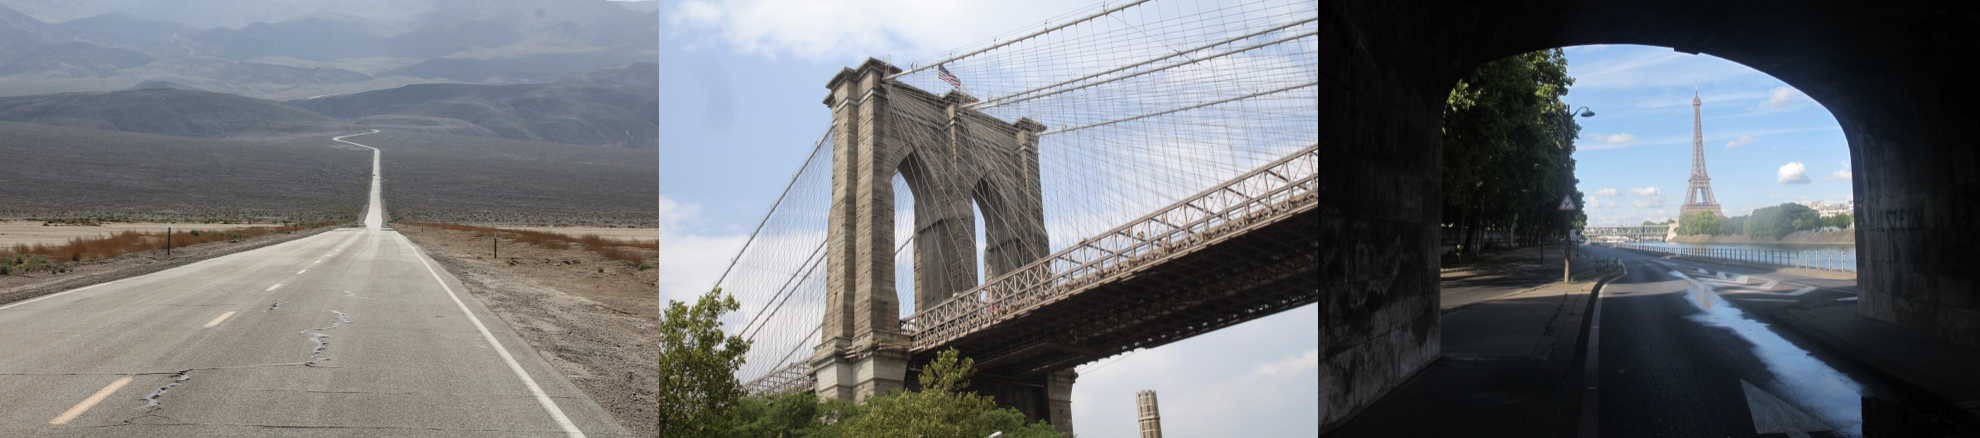
\includegraphics[width=1\linewidth]{cnn/landmarks-example.png}
\captionof{figure}{Examples from the landmarks dataset - a road in Death Valley, the Brooklyn Bridge, and the Eiffel Tower}


\section{Project Steps}

The high level steps of the project include:

\begin{enumerate}
    \item \textit{Create a CNN to Classify Landmarks (from Scratch)} - Here, you'll visualize the dataset, process it for training, and then build a convolutional neural network from scratch to classify the landmarks. You'll also describe some of your decisions around data processing and how you chose your network architecture. You will then export your best network using Torch Script.
    \item \textit{Create a CNN to Classify Landmarks (using Transfer Learning)} - Next, you'll investigate different pre-trained models and decide on one to use for this classification task. Along with training and testing this transfer-learned network, you'll explain how you arrived at the pre-trained network you chose. You will also export your best transfer learning solution using Torch Script
    \item \textit{Deploy your algorithm in an app} - Finally, you will use your best model to create a simple app for others to be able to use your model to find the most likely landmarks depicted in an image. You'll also test out your model yourself and reflect on the strengths and weaknesses of your model.
\end{enumerate}
Each of these three major steps is carried out in a corresponding Jupyter Notebook that you will be provided in the project starter kit. So there are three notebooks that will guide you in your project work.

\subsection{Starter Code and Instructions}

Starter code is provided to you in the project workspace, and is also available for you to download if you prefer to work locally. Please follow the detailed instructions contained in the following three notebooks:

\begin{enumerate}
    \item \textit{cnn\_from\_scratch.ipynb}: Create a CNN from scratch
    \item \textit{transfer\_learning.ipynb}: Use transfer learning
    \item \textit{app.ipynb}: Deploy your best model in an app. At the end of this notebook you will also generate the archive file that you will submit for review
\end{enumerate}

\subsection{Evaluation}

Your project will be reviewed by a Udacity reviewer against the \href{https://learn.udacity.com/rubric/4814}{\textbf{project rubric}}. Review this rubric thoroughly, and evaluate your project against the rubric before submission. Your project must satisfy every criterion in the rubric for you to pass.

We have also written some tests for each step of the process to help you self-diagnose the most common problems. You will be running these tests as part of the development process, as described in the notebooks. Do not skip ahead if the tests are not passing. When tests fail, they will usually provide some clear guidance on what went wrong.

\subsection{Project Submission}

At the end of the \verb|app.ipynb| notebook there are instructions on how to generate a file with a name like \verb|submission_2022-03-31T00h55m.tar.gz| that contains all your notebooks and code. If you worked in the Project Workspace, you will download that file from the workspace to your machine. If you worked locally the file will already be on your machine, in the same directory as the notebooks. After you have obtained the file, go to the Project Submission page and submit it.


\section{Environment and Dependencies [WORKSPACE OR LOCAL]}

\subsection{Environment and Dependencies}

For this project, you can either complete the work on your own local computer or you can complete it within a workspace right here in the Udacity classroom.

\subsubsection{Option 1: Working in the Udacity project workspace}

You can find the Udacity Project Workspace here in your Udacity classroom, on the Project Workspace page.

On the workspace page, when prompted on whether you want a GPU or not, please ANSWER YES (the GPU is going to make everything several times faster).

The environment is already set up for you, including the starter code, so you can jump right into building your project!

\subsubsection{Option 2: Working locally}

Alternatively, you can develop your project locally on your computer. This setup requires a bit of familiarity with creating a working deep learning environment. While things should work out of the box, in case of problems you might have to do operations on your system (like installing new NVIDIA drivers for your GPU) that are not covered in the class. Please work on your local environment only if you are at least a bit familiar with these subjects, otherwise we recommend using the provided Udacity workspace in the classroom.

\begin{enumerate}
    \item Download the starter kit from the Resources section of the left sidebar of the Udacity classroom here. (Scroll down if you don't see it.)
    \item Open a terminal and navigate to the directory where you installed the starter kit.
    \item Download and install \href{https://docs.conda.io/en/latest/miniconda.html}{\textbf{Miniconda}}
    \item Create a new conda environment with Python 3.7.6:
\end{enumerate}

\begin{verbatim}
\verb|conda create --name udacity python=3.7.6 pytorch=1.11.0 torchvision torchaudio cudatoolkit -c pytorch|
\end{verbatim}

Activate the environment:

\begin{verbatim}
\verb|conda activate udacity|
\end{verbatim}

NOTE: You will need to activate your environment again every time you open a new terminal.

Install the required packages for the project:

\begin{verbatim}
\verb|pip \textbf{install} -r requirements.txt|
\end{verbatim}

Test that the GPU is working (execute this only if you have a NVIDIA GPU on your machine, which Nvidia drivers properly installed)

\begin{verbatim}
\verb|python -c "import torch;print(torch.cuda.is_available())|
\end{verbatim}

This should return \verb|True|. If it returns \verb|False| your GPU cannot be recognized by pytorch. Test with \verb|nvidia-smi| that your GPU is working. If it is not, check your NVIDIA drivers. If you cannot solve this problem, please consider using the Project Workspace instead of working locally.

Install and open jupyter lab:

\begin{verbatim}
\verb|pip \textbf{install} jupyterlab jupyter lab|
\end{verbatim}
